\section{Results}

\begin{frame}
    \frametitle{Results - Loss curves}

    \begin{center}
        
        \begin{figure}[H]
            \centering
            \begin{subfigure}[b]{0.45\textwidth}
                \centering
                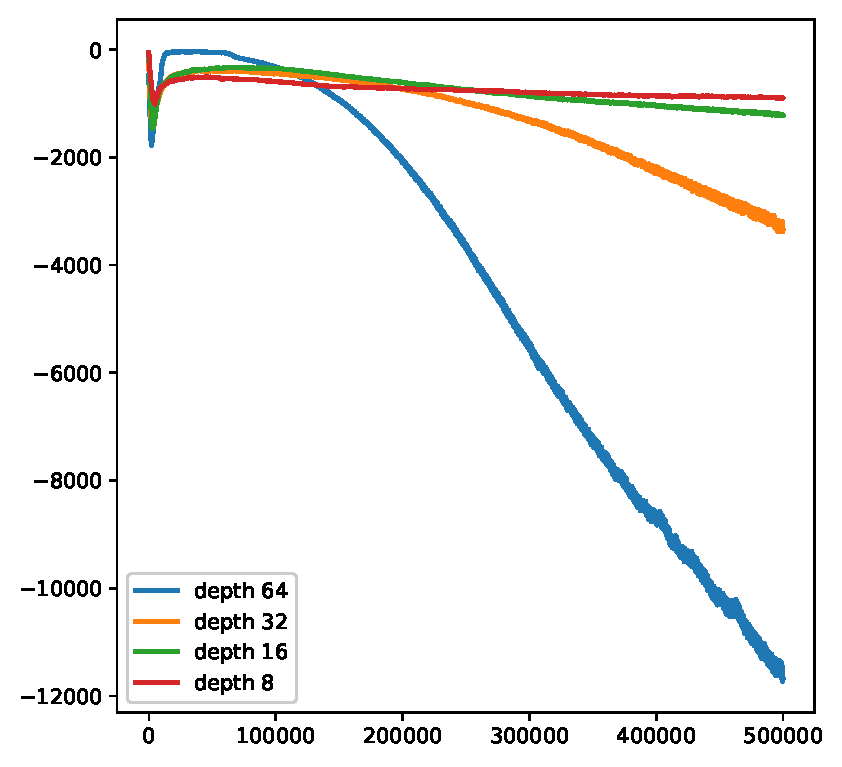
\includegraphics[width=\textwidth]{resources/images/celeba_hq_d_loss.eps}
                \caption{Anime Face}
                \label{fig:celeba_hq_d_loss}
            \end{subfigure}
            \hfill
            \begin{subfigure}[b]{0.45\textwidth}
                \centering
                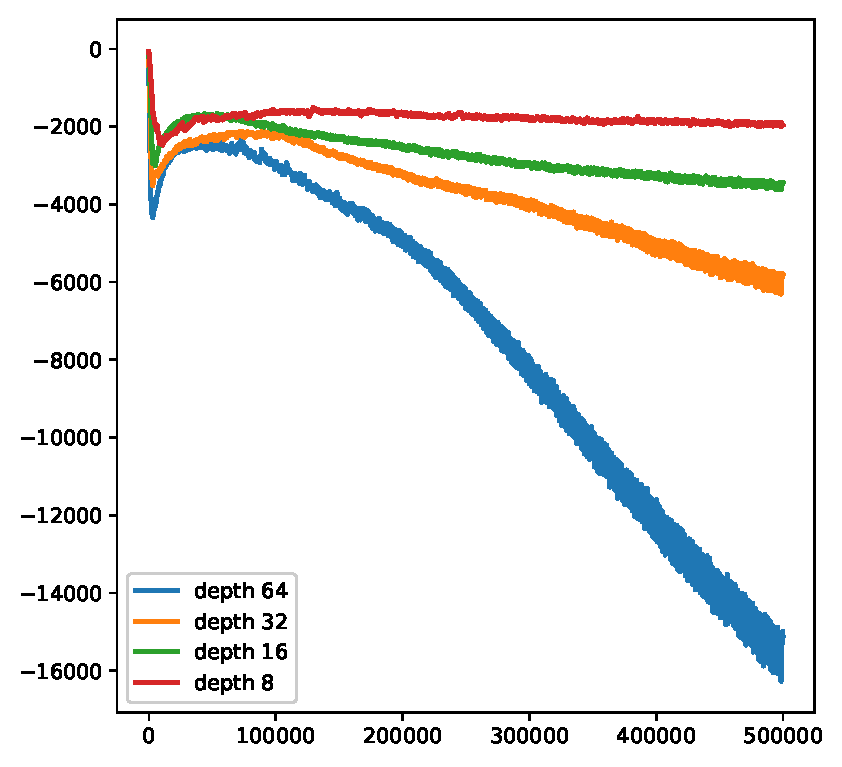
\includegraphics[width=\textwidth]{resources/images/anime_face_d_loss.eps}
                \caption{CelebA HQ}
                \label{fig:anime_face_d_loss}
            \end{subfigure}
            \caption{Discriminator loss curves}
            \label{fig:d_loss}
        \end{figure}
                
    \end{center}
\end{frame}

\begin{frame}
    \frametitle{Results - Samples Celeba HQ}

    \begin{center}
    
        \begin{figure}[H]
            \centering
            \begin{subfigure}[b]{0.24\textwidth}
                \centering
                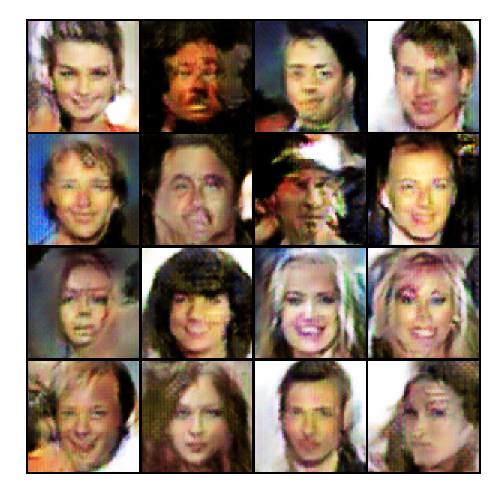
\includegraphics[width=\textwidth]{resources/images/output_celeba_8.eps}
                \caption{depth 8}
                \label{fig:celeba_8}
            \end{subfigure}
            \hfill
            \begin{subfigure}[b]{0.24\textwidth}
                \centering
                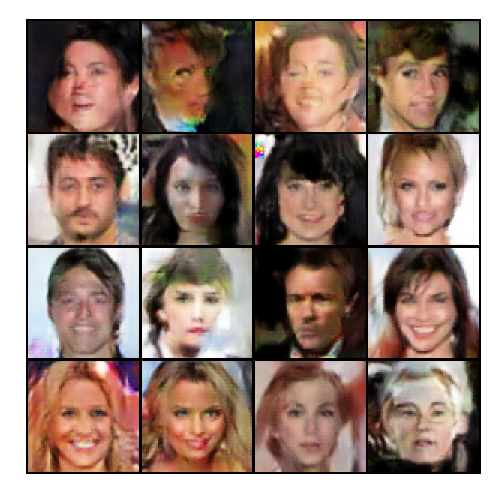
\includegraphics[width=\textwidth]{resources/images/output_celeba_16.eps}
                \caption{depth 16}
                \label{fig:celeba_16}
            \end{subfigure}
            \hfill
            \begin{subfigure}[b]{0.24\textwidth}
                \centering
                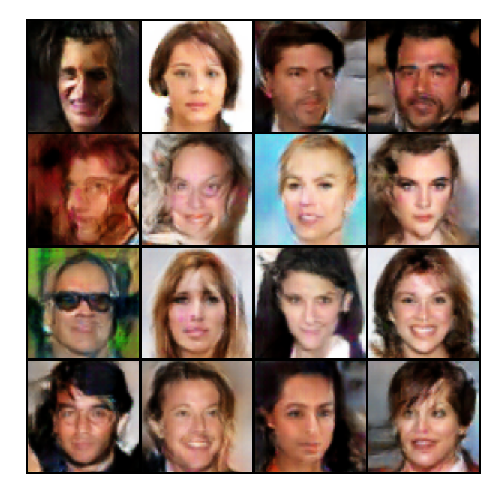
\includegraphics[width=\textwidth]{resources/images/output_celeba_32.eps}
                \caption{depth 32}
                \label{fig:celeba_32}
            \end{subfigure}
            \hfill
            \begin{subfigure}[b]{0.24\textwidth}
                \centering
                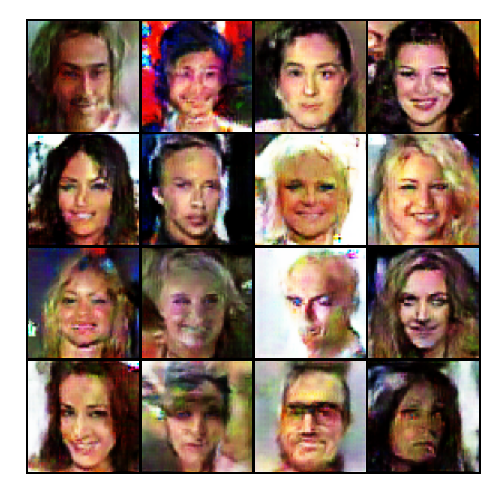
\includegraphics[width=\textwidth]{resources/images/output_celeba_64.eps}
                \caption{depth 64}
                \label{fig:celeba_64}
            \end{subfigure}
            \caption{Sample generated images of different models trained on the Celeba HQ dataset}
            \label{fig:output_celeba}
        \end{figure}
    
    \end{center}
\end{frame}

\begin{frame}
    \frametitle{Results - Samples Anime Face}

    \begin{center}
    
        \begin{figure}[H]
            \centering
            \begin{subfigure}[b]{0.24\textwidth}
                \centering
                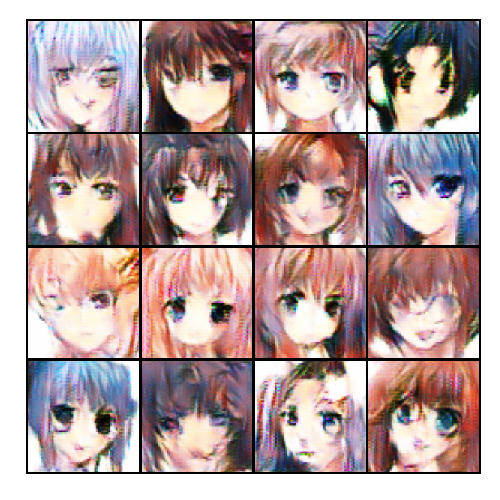
\includegraphics[width=\textwidth]{resources/images/output_anime_8.eps}
                \caption{depth 8}
                \label{fig:anime_8}
            \end{subfigure}
            \hfill
            \begin{subfigure}[b]{0.24\textwidth}
                \centering
                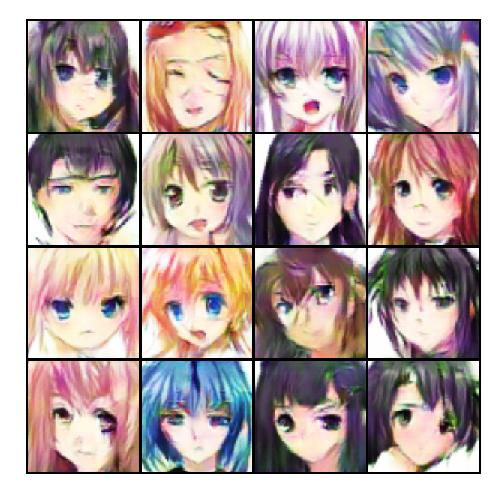
\includegraphics[width=\textwidth]{resources/images/output_anime_16.eps}
                \caption{depth 16}
                \label{fig:anime_16}
            \end{subfigure}
            \hfill
            \begin{subfigure}[b]{0.24\textwidth}
                \centering
                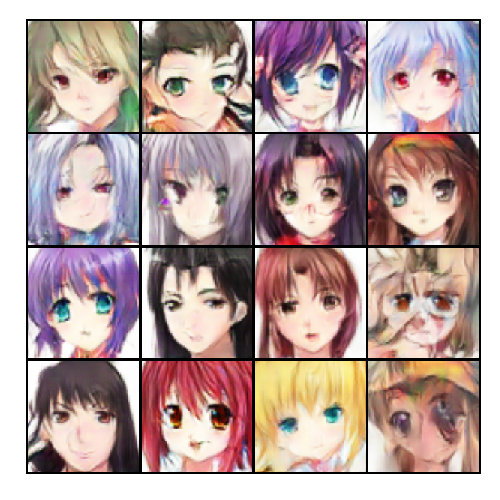
\includegraphics[width=\textwidth]{resources/images/output_anime_32.eps}
                \caption{depth 32}
                \label{fig:anime_32}
            \end{subfigure}
            \hfill
            \begin{subfigure}[b]{0.24\textwidth}
                \centering
                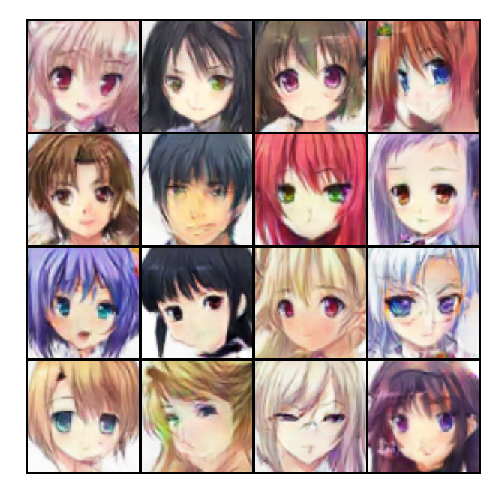
\includegraphics[width=\textwidth]{resources/images/output_anime_64.eps}
                \caption{depth 64}
                \label{fig:anime_64}
            \end{subfigure}
            \caption{Sample generated images of different models trained on the Anime Face dataset}
            \label{fig:ouput_anime}
        \end{figure}

    
    \end{center}
\end{frame}

\begin{frame}
    \frametitle{Conclusion}

    \begin{center}
        \begin{itemize}
            \item Proposed framework is able to generate RGB-Images
            \item Still has artifacts
            \item Training can become unstable 
            \item Small image size
            \item Gradient penalty slows down the training
        \end{itemize}
    \end{center}
\end{frame}

\begin{frame}
    \frametitle{Conclusion - Future work}

    \begin{center}
            \begin{itemize}
                \item Skip-connections \cite{karnewar2020msggan}
                \item Better loss function \cite{realness} \cite{jolicoeurmartineau2018rahinge}, architecture
                \item Image-to-Image translation \cite{cyclegan}
                \item More controll over generated images \cite{stylegan}, \cite{stylegan2}
            \end{itemize}
    \end{center}
\end{frame}